% figoverview.tex

\usetikzlibrary{shapes,arrows, positioning}

% Define block styles
\tikzstyle{block} = [rectangle, draw, fill=blue!20, text centered, minimum height=2em, node distance=2cm]
\tikzstyle{line} = [draw, -latex']
	
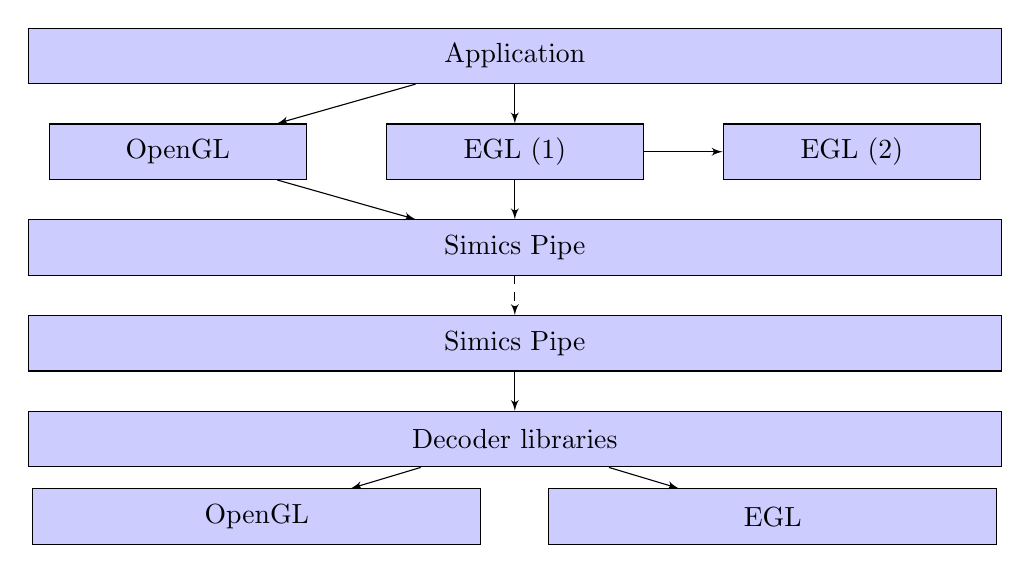
\begin{tikzpicture}
	\node[block, text width=\linewidth, align=center] (app) {Application};
	
	\node[block, below=0.5cm of app, text width=0.25\linewidth] (targetegl) {EGL (1)};
	\node[block, left=1cm of targetegl, text width=0.25\linewidth] (targetgl) {OpenGL};
	\node[block, right=1cm of targetegl, text width=0.25\linewidth] (targeteglnative) {EGL (2)};
	
	\node[block, text width=\linewidth, below=0.5cm of targetegl] (pipetarget) {Simics Pipe};
	\node[block, text width=\linewidth, below=0.5cm of pipetarget] (pipehost) {Simics Pipe};

	\node[block, text width=\linewidth, below=0.5cm of pipehost] (hostlibraries) {Decoder libraries};
	
	\node[below=0.5cm of hostlibraries] (dummy) {};
	\node[block, text width=0.45\linewidth, left=0.3cm of dummy] (hostgl) {OpenGL};
	\node[block, text width=0.45\linewidth, right=0.3cm of dummy] (hostegl) {EGL};

	\path [line] (app) -- (targetgl);
	\path [line] (app) -- (targetegl);
	\path [line] (targetegl) -- (targeteglnative);

	\path [line] (targetgl) -- (pipetarget);
	\path [line] (targetegl) -- (pipetarget);

	\path [line, dashed] (pipetarget) -- (pipehost);

	\path [line] (pipehost) -- (hostlibraries);

	\path [line] (hostlibraries) -- (hostgl);
	\path [line] (hostlibraries) -- (hostegl);
\end{tikzpicture}
